\chapter*{Introduction}		
\addcontentsline{toc}{chapter}{Introduction}	%добавляем в оглавление			
FAINA - is a numerical code for modeling different types of electromagnetic radiation of astrophysical source. It is written in C++ and supports parallel computations using openmp method. FAINA allows to model observable fluxes from sources with different parameters and geometries vai different emission mechanisms, and also to optimize source parameters to fit observational data.

\section*{Installation}
\addcontentsline{toc}{section}{Installation}
Current version of the code is available on github https://github.com/VadimRomansky/Faina. FAINA is distributed freely under the MIT public license. Download the archive with code and extract it into preferred root directory.

\subsection*{Windows}
\addcontentsline{toc}{subsection}{Windows}
With Windows OS it is recomended to use Microsoft Visual Studio and open solution Faina.sin with it. Operability was examined for Windows 10 and Visual Studio 2022 version.

\subsection*{Unix}
\addcontentsline{toc}{subsection}{Unix}
There are two possible ways to run FAINA on Unix. We recommend to use IDE QtCreator and open  with it file Faina.pro located in the rrot directory.

Other way is to use FAINA from terminal. To compile and run it you can use following commands

\begin{lstlisting}[language=bash]
	$ g++ -o faina *.cpp
	$ ./faina
\end{lstlisting}

Operability was examined for Ubuntu 22.04.

\section*{Runnng simple problem}\label{running}
\addcontentsline{toc}{section}{Runnng simple problem}

Let see a simple example of solving radiation problem with faina. You can find in the function evaluateSimpleSynchrotron in the file /Src/examples.cpp. Synchrotron radiation from homogenous source with   the shape of cylinder with axis along line of sight and with powerlaw electron distribution is evaluated in this example. But it demonstrates a general approach to evaluation of radiation with FAINA code.

Let define values of magnetic field and electron number density in the source (code uses CGS units).

\begin{lstlisting}[language=c++]
	double B = 1.0;
	double electronConcentration = 1.0;
\end{lstlisting}

Then you need to create distribution of emitting electrons. There are a different type of particle distribution implemented in the code, let use isotropic powerlaw distribution for this example. You should call the constructor of MassiveParticlePowerLawDistribution with following parameters - mass of emitting particles (electrons in this case), powerlaw index of distribution, which is defined as positive number $p$ in $F(E) ~ 1/E^p$, starting energy of powerlaw distribution, and electrons number density. 

\begin{lstlisting}[language=c++]
	MassiveParticleDistribution* distribution =
	new MassiveParticlePowerLawDistribution(
	massElectron, 3.0, me_c2, electronConcentration);
\end{lstlisting}

After that you should create a radiation source, for example it would be homogenous flat disk with axis along line of sight. You should call the constructor of SimpleFlatSource with following parameters: electrons distribution, magnetic field, sinus of it's inclination angle to the line of sight, radous of cylinder, it's hight and distance to the observer.

\begin{lstlisting}[language=c++]
	RadiationSource* source = new SimpleFlatSource(
	distribution, B, 1.0, parsec, parsec, 1000 * parsec);
\end{lstlisting}

And the last thing you need is an radiation evaluator. They are different for every specific type of radiation. Here we create a SybchrotronEvaluator with following parameters: number of grid points for integration electron distribution function over energy, lower and upper limits of electron energy that will be taken into account and boolean parameter determining include synchrotron self absorption or not.

\begin{lstlisting}[language=c++]
	RadiationEvaluator* evaluator = new 
	SynchrotronEvaluator(1000, me_c2, 1000 * me_c2, true);
\end{lstlisting}

Synchrotron approximation is valid only for frequencies of radiation much greater than cyclotron frequency, so let evaluate it

\begin{lstlisting}[language=c++]
	double cyclOmega = 
	electron_charge * B / (massElectron * speed_of_light);
\end{lstlisting}

Now you can evaluate spectrum of synchrotron radiation. Radiation evaluator has a method writeFluxFromSourceToFile which allows to calculate flux energy density and write it into the file in units energy vs power per energy per area, or $\rm erg$ vs $\rm sm^-2 s^-1$. This method takes following input parametes: output file name which will be created or rewritten, lower and upper limits of energy range and number of grid points, which will be distributed logarithmically in the range. If you need other units you should use method evaluateFluxFromSource which provides a flux energy density at given energy and rewrite output.

\begin{lstlisting}[language=c++]
	evaluator->writeFluxFromSourceToFile("out.dat",source, 
	10*hplank*cyclOmega, 1E5*hplank*cyclOmega, 1000);
\end{lstlisting}


Evaluated spectrum of flux energy density from this source is shown in \ref{example0}. Examples of plotting scripts you can find in Figure directory pyFAINA.
\begin{figure}
	\centering
	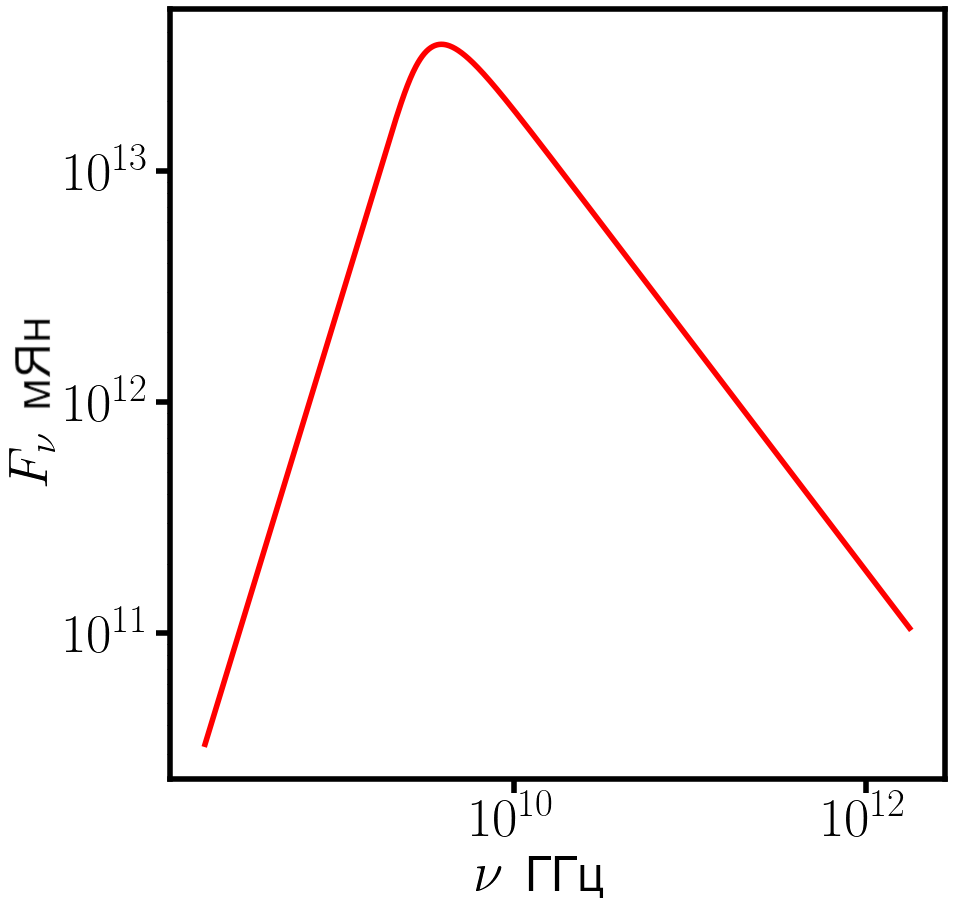
\includegraphics[width=12.5 cm]{./fig/example0.png} 
	\caption{Synchrotron radiation flux energy density from test source}
	\label{example0}
\end{figure}